%%%%%%%%%%%%%%%%%%%%%%%%%%%%%%%%%%%%%%%%%%%%%%%%%%%%%%%%%%%%%%%%%%%%%%%%%%%%%%%
%  CARLTON FL: Federated Deep Reinforcement Learning for Distributed Channel
%  Allocation in Cognitive Interference Networks
%  Compile with: pdflatex (twice)
%%%%%%%%%%%%%%%%%%%%%%%%%%%%%%%%%%%%%%%%%%%%%%%%%%%%%%%%%%%%%%%%%%%%%%%%%%%%%%%
\documentclass[journal]{IEEEtran}

\usepackage{amsmath,amssymb,amsfonts}
\usepackage{graphicx}
\usepackage{booktabs}
\usepackage{xcolor}
\usepackage{tikz}
\usetikzlibrary{arrows.meta,positioning,fit,backgrounds,calc,shapes.geometric}
\usepackage{url}
\usepackage{algorithm}
\usepackage{algpseudocode}
\usepackage[hidelinks]{hyperref}

\graphicspath{{figs/}}

\newcommand{\CARLTON}{\textsc{Carlton}}
\newcommand{\OURS}{\textsc{Carlton\,FL}}
\newcommand{\FedAvg}{\textsc{FedAvg}}
\newcommand{\FedProx}{\textsc{FedProx}}

\begin{document}

\title{\textsc{Carlton FL}: Federated Deep Reinforcement Learning for\\
Distributed Channel Allocation in Cognitive\\
Interference Networks}

\author{Tomer~Baziza,
        Yaniv~Cohen,
        and~Kobi~Cohen,~\IEEEmembership{Senior Member,~IEEE}%
\thanks{T.~Baziza is with the School of Electrical and Computer Engineering,
Ben-Gurion University of the Negev, Beer-Sheva 8410501, Israel.}%
\thanks{Y.~Cohen is a research assistant with the School of Electrical and
Computer Engineering, Ben-Gurion University of the Negev.}%
\thanks{K.~Cohen is with the School of Electrical and Computer Engineering,
Ben-Gurion University of the Negev (corresponding author:
\texttt{yakovsec@bgu.ac.il}).}}

\maketitle

%==============================================================================
\begin{abstract}
%------------------------------------------------------------------------------
We consider distributed dynamic channel allocation (DCA) in cognitive
interference networks, where a shared band is divided into $K$ non-orthogonal
channels and inter-carrier interference (ICI) couples the decisions of
spatially overlapping networks. State-of-the-art deep reinforcement learning
(DRL) solutions for this setting operate under the \emph{centralized training
with decentralized execution} (CTDE) paradigm: although execution is
distributed, training requires every network to export its raw sensing history
to a shared replay memory and concentrates all gradient computation on a single
learner. We propose \OURS{}, a federated DRL framework that removes the
centralized learner altogether. Each network manager acts as a federated client
that owns a private, persistent replay buffer, performs $E$ local update steps
of a target-network-free mellowmax value learner, and uploads only model
parameters, which a server aggregates by \FedAvg{} or \FedProx{}. We identify
three sources of statistical heterogeneity that are specific to federated DRL
for DCA---topological asymmetry, policy-induced non-stationarity, and
inter-agent coupling---and show that the \FedProx{} proximal term is what keeps
long local phases stable under them. Over $30$ seeds, $1000$ training rounds,
and $100$ frozen-weight inference episodes, \OURS{} with \FedProx{}
$(E{=}10,\mu{=}0.01)$ attains an inference reward of $86.64\pm 1.01$, against
$78.91\pm 0.73$ for the centralized TensorFlow CTDE baseline and
$78.99\pm 0.79$ for its PyTorch counterpart---while raw sensing data never
leaves the network that produced it. On the operational channel-quality
metrics of the centralized state of the art
($\mathbb{E}[(\mathrm{CQ}+\min\mathrm{CQ})/2]$ and WS), the centralized
PyTorch CTDE baseline leads slightly ($0.909$ all-sample composite versus
$0.905$ for \FedProx{}), while \OURS{} remains in the same operating regime
under a strictly stronger privacy constraint.
\end{abstract}

\begin{IEEEkeywords}
Federated learning, deep reinforcement learning, distributed dynamic channel
allocation (DCA), cognitive interference networks, inter-carrier interference
(ICI), signal-to-interference-plus-noise ratio (SINR), non-IID data.
\end{IEEEkeywords}

%==============================================================================
\section{Introduction}
\label{sec:intro}
%==============================================================================

\IEEEPARstart{T}{he} growing demand for wireless connectivity, together with
spectrum scarcity, has made \emph{dynamic channel allocation} (DCA) a central
mechanism in emerging cognitive communication systems. In contrast to static
allocation, DCA lets every network revise its operating channel in response to
the interference it currently experiences. The mechanism is relevant across
cognitive radio networks, 6G in-X sub-networks, vehicular ad-hoc networks,
wireless sensor and IoT networks, and wireless mesh networks---all
characterized by dense coexistence of independently managed networks within a
shared band~\cite{cohen2024carlton}.

Most existing formulations simplify the problem by assuming perfectly
orthogonal channels, so that interference occurs only between networks
occupying the \emph{same} channel. This assumption rarely holds in practice.
Spectral leakage and hardware imperfections produce \emph{inter-carrier
interference} (ICI), and partially overlapping channels measurably affect
network performance~\cite{mishra2006overlapped}. Once orthogonality is dropped,
a channel is interfered with not only by co-channel transmissions but also, to
a degree decaying with spectral distance, by every neighboring channel. The
resulting coupling is continuous rather than binary, varies over the network
graph with geographic distance, and inflates the search space to the point
where classical allocation algorithms become inefficient.

Four properties make distributed DCA under ICI particularly difficult. First,
each network manager observes only its own sensing measurements and therefore
holds a strictly partial view of the global interference state, placing the
problem in the class of partially observable Markov decision processes.
Second, the environment is non-stationary: when one manager switches channel,
the observation and reward distributions of all of its neighbors change
simultaneously. Third, the optimal joint assignment generalizes graph coloring
to weighted, non-binary interference and is
intractable~\cite{blum2003metaheuristics}; it cannot be recomputed centrally at
the timescale on which topologies evolve. Fourth, spectrum mobility is itself
costly, since every reallocation interrupts service, so a useful policy must
converge quickly and then remain stable.

%------------------------------------------------------------------------------
\subsection{DRL Algorithms for DCA}
\label{subsec:intro_related}
%------------------------------------------------------------------------------

Multi-agent DRL is an attractive framework for DCA precisely because it
requires no explicit model of the interference environment: agents learn a
channel-selection policy directly from interaction and implicitly discover the
spatial reuse structure of the network. Following the early multi-user DRL work
of Naparstek and Cohen~\cite{naparstek2019deep}, a substantial line of research
has applied deep $Q$-learning and its variants to spectrum
access~\cite{adeogun2023distributed,kaur2023deep,du2022multi}. The current
state of the art for the SINR-aware setting considered here is
\CARLTON{}~\cite{cohen2024carlton}, which reports gains of roughly $45\%$ over
a random-agent benchmark~\cite{cohen2017distributed} and $20\%$ over the
Jamming Avoidance Response (JAR) heuristic, outperforms the DRL baselines
MADDQN-DCA~\cite{adeogun2023distributed} and IDSA~\cite{kaur2023deep}, and
comes within about $2.5\%$ of a centralized graph-coloring upper bound. It is
the benchmark against which we position our framework.

What all of these methods share---and what this paper targets---is their
\emph{training} architecture. Although the learned policies execute in a fully
distributed manner, with no controller and no message exchange between networks
at test time, they are trained under the CTDE paradigm, illustrated in
Fig.~\ref{fig:paradigms}(a): during an episode each network manager $n$ writes
its transitions into a small local memory $\mathcal{D}^{n}$ holding its $T$
decision points; at the end of the episode every $\mathcal{D}^{n}$ is flushed
into a global replay memory (GRM) of capacity $S_{z}$, and one central learner
draws mini-batches from the GRM and performs all gradient updates. The local
buffers are mere staging areas; the learning signal is entirely centralized.

This imposes three limitations that are decisive in practice. \emph{Privacy and
data sovereignty}: every transition contains the agent's quality vector, which
encodes fine-grained information about its spectral environment, its
interference neighborhood, and---by implication---its physical location, its
number of active users, and its traffic behavior; exporting it is unacceptable
when the participating networks belong to competing operators, distinct
tactical units, or different regulatory domains. \emph{Computational
centralization}: all gradient computation is performed by one node, which
becomes both a scalability bottleneck and a single point of failure, while the
network managers---which the system model already assumes to be capable
computing nodes---remain idle. \emph{Deployment realism}: independently
operated networks rarely accept a common trusted training authority. There is a
genuine tension here, since the case for distributed DCA is made precisely on
the grounds of communication overhead and computational
complexity~\cite{cohen2024carlton}, yet those same costs reappear in the
training phase.

Federated learning~\cite{mcmahan2017fedavg,kairouz2021advances} is the natural
answer, but transplanting it into multi-agent DRL for DCA is not mechanical.
In supervised federated learning the client datasets are fixed and non-IID only
through their label distributions. Here each client \emph{generates} its own
data with the policy it is currently learning, inside an environment whose
other occupants are the remaining clients. The heterogeneity is consequently
structural, non-stationary, and coupled---the regime in which plain parameter
averaging is known to be fragile.

%------------------------------------------------------------------------------
\subsection{Main Results}
\label{subsec:intro_main}
%------------------------------------------------------------------------------

We develop \OURS{}, a federated DRL framework for SINR-aware distributed DCA
under ICI, shown in Fig.~\ref{fig:paradigms}(b). The global replay memory is
eliminated: each network manager is a federated client owning a
\emph{persistent} private buffer, retained across episodes rather than flushed
to a central store. A round proceeds in four phases---the server broadcasts
$w^{t}$; each client plays one interaction episode; each client performs $E$
local gradient steps on samples drawn exclusively from its own buffer; each
client uploads only $w^{t+1}_{n}$, which the server aggregates. Raw experience
never leaves the client, and once training terminates the server is no longer
needed. Our contributions are as follows.

\textbf{C1. A federated DRL framework for SINR-aware DCA under ICI.} To the
best of our knowledge, this is the first federated reinforcement learning
framework for distributed channel allocation in cognitive interference networks
with non-orthogonal channels. We show that the episodic transfer of experience
into a global replay memory---the mechanism on which the centralized state of
the art relies---can be replaced by persistent per-agent buffers with
parameter-level aggregation, without altering the observation space, the action
space, or the message-free execution phase. We release a complete open-source
implementation together with a faithful reproduction of the centralized
baseline, so that the two paradigms differ only in how learning is coordinated.

\textbf{C2. Taming non-IID multi-agent experience with \FedProx{}.} We
characterize three sources of statistical heterogeneity specific to federated
DRL for DCA---topological and load asymmetry across agents, policy-induced
non-stationarity of each local buffer, and inter-agent coupling of the local
objectives---and show that together they make client drift the dominant failure
mode when the number of local steps is large. We adopt the \FedProx{} proximal
objective and conduct a systematic sweep over the local-epoch count $E$ and the
proximal coefficient $\mu$, identifying $E^{\star}=10$ and $\mu^{\star}=0.01$
as the configuration that best balances communication efficiency against
stability.

\textbf{C3. Privacy-preserving training that remains competitive with CTDE.}
All SINR measurements, quality vectors, user counts, and transition tuples
remain in the network that generated them; only model parameters cross the
network boundary, and the training computation is distributed across the
network managers. Across $30$ seeds, \OURS{} reaches an inference reward of
$86.64\pm 1.01$ (\FedProx{}) and $86.47\pm 1.21$ (\FedAvg{}). We treat the
reward as a training proxy rather than as a claim of superiority over CTDE:
federated clients train under a stricter information constraint ($\rho=1$, no
social term) and the primary evaluation uses the same channel-quality metrics
as the centralized state of the art. The experimental finding is that private,
persistent buffers with parameter averaging are sufficient to keep federated
DRL competitive with \CARLTON{} on this task.

The remainder of this paper is organized as follows.
Section~\ref{sec:model} formalizes the system model and the constrained DCA
objective, and maps them onto a federated optimization problem.
Section~\ref{sec:method} presents the \OURS{} algorithm.
Section~\ref{sec:experiments} reports the experimental study, and
Section~\ref{sec:conclusion} concludes.

%------------------------------------------------------------------------------
% FIGURE: CTDE vs FRL
%------------------------------------------------------------------------------
\begin{figure*}[!t]
\centering
\resizebox{0.92\textwidth}{!}{%
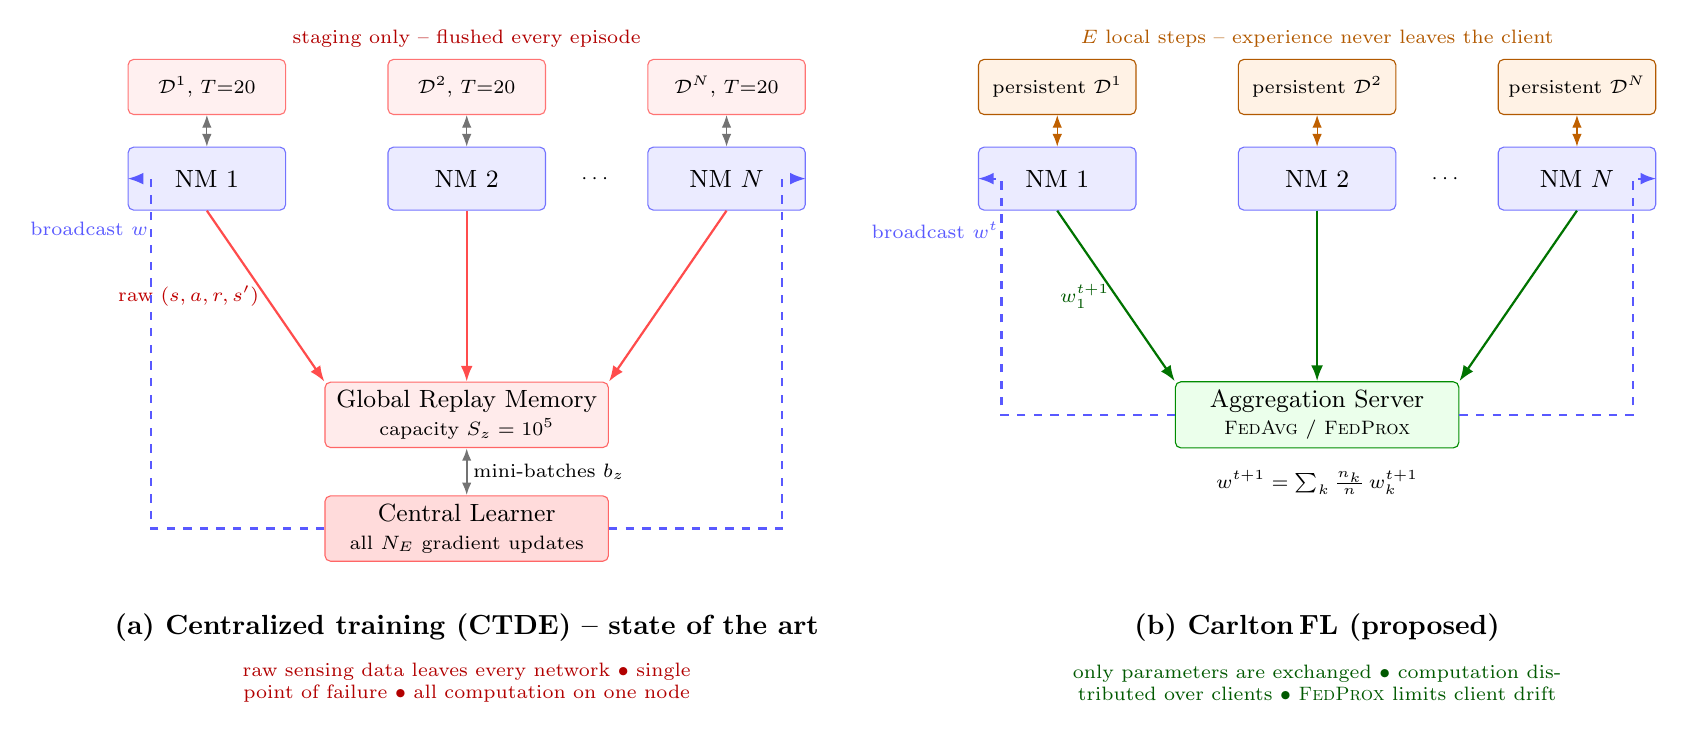
\begin{tikzpicture}[
  font=\small,
  box/.style   = {rounded corners=2pt, draw=black!65, fill=white,
                  minimum width=20mm, minimum height=8mm, align=center,
                  inner sep=3pt},
  agent/.style = {box, fill=blue!8, draw=blue!55},
  serverc/.style= {box, fill=red!8, draw=red!60, minimum width=36mm},
  serverf/.style= {box, fill=green!8, draw=green!55!black, minimum width=36mm},
  bufc/.style  = {box, fill=red!6, draw=red!55, font=\scriptsize,
                  minimum width=20mm, minimum height=7mm},
  buff/.style  = {box, fill=orange!10, draw=orange!70!black, font=\scriptsize,
                  minimum width=20mm, minimum height=7mm},
  raw/.style   = {-{Latex[length=2mm]}, draw=red!70, thick},
  wgt/.style   = {-{Latex[length=2mm]}, draw=green!45!black, thick},
  bcast/.style = {-{Latex[length=2mm]}, draw=blue!65, thick, dashed},
  loc/.style   = {{Latex[length=1.6mm]}-{Latex[length=1.6mm]}, draw=black!55},
  lbl/.style   = {font=\scriptsize, inner sep=1pt}
]

%%%%%%%%%%%%%%%%%%%%%%% (a) CENTRALIZED CTDE %%%%%%%%%%%%%%%%%%%%%%%%%%%%%%%%%
\begin{scope}
  \node[serverc] (grm) at (0,0) {Global Replay Memory\\[-1pt]
        {\scriptsize capacity $S_z=10^{5}$}};
  \node[serverc, below=6mm of grm, fill=red!14] (learner)
        {Central Learner\\[-1pt]{\scriptsize all $N_E$ gradient updates}};

  \node[agent] (a1) at (-3.3,3.0) {NM $1$};
  \node[agent] (a2) at ( 0.0,3.0) {NM $2$};
  \node[agent] (a3) at ( 3.3,3.0) {NM $N$};
  \node[lbl]   at (1.65,3.0) {$\cdots$};

  \node[bufc, above=4mm of a1] (d1) {$\mathcal{D}^{1}$, $T{=}20$};
  \node[bufc, above=4mm of a2] (d2) {$\mathcal{D}^{2}$, $T{=}20$};
  \node[bufc, above=4mm of a3] (d3) {$\mathcal{D}^{N}$, $T{=}20$};
  \draw[loc] (a1) -- (d1);  \draw[loc] (a2) -- (d2);  \draw[loc] (a3) -- (d3);
  \node[lbl, red!70!black, above=1mm of d2] {staging only -- flushed every episode};

  \draw[raw] (a1.south) -- node[lbl,left=1pt,pos=0.5]
        {\textcolor{red!75!black}{raw $(s,a,r,s')$}} (grm.north west);
  \draw[raw] (a2.south) -- (grm.north);
  \draw[raw] (a3.south) -- (grm.north east);

  \draw[loc, thick] (grm.south) -- node[lbl,right=1pt]
        {\scriptsize mini-batches $b_z$} (learner.north);

  \draw[bcast] (learner.west) -- ++(-2.2,0) |- (a1.west);
  \draw[bcast] (learner.east) -- ++( 2.2,0) |- (a3.east);
  \node[lbl, blue!65, below left=1mm and -3mm of a1.south west]
        {broadcast $w$};

  \node[font=\bfseries] at (0,-2.7) {(a) Centralized training (CTDE) -- state of the art};
  \node[lbl, text width=68mm, align=center, red!70!black] at (0,-3.4)
        {raw sensing data leaves every network~$\bullet$~single point of
         failure~$\bullet$~all computation on one node};
\end{scope}

%%%%%%%%%%%%%%%%%%%%%%% (b) FEDERATED FRL %%%%%%%%%%%%%%%%%%%%%%%%%%%%%%%%%%%%
\begin{scope}[xshift=108mm]
  \node[serverf] (agg) at (0,0)
        {Aggregation Server\\[-1pt]{\scriptsize \FedAvg{} / \FedProx{}}};
  \node[below=1.5mm of agg, font=\scriptsize, align=center]
        {$w^{t+1}=\sum_{k}\frac{n_k}{n}\,w_k^{t+1}$};

  \node[agent] (b1) at (-3.3,3.0) {NM $1$};
  \node[agent] (b2) at ( 0.0,3.0) {NM $2$};
  \node[agent] (b3) at ( 3.3,3.0) {NM $N$};
  \node[lbl]   at (1.65,3.0) {$\cdots$};

  \node[buff, above=4mm of b1] (p1) {persistent $\mathcal{D}^{1}$};
  \node[buff, above=4mm of b2] (p2) {persistent $\mathcal{D}^{2}$};
  \node[buff, above=4mm of b3] (p3) {persistent $\mathcal{D}^{N}$};
  \draw[loc, draw=orange!75!black] (b1) -- (p1);
  \draw[loc, draw=orange!75!black] (b2) -- (p2);
  \draw[loc, draw=orange!75!black] (b3) -- (p3);
  \node[lbl, orange!70!black, above=1mm of p2]
        {$E$ local steps -- experience never leaves the client};

  \draw[wgt] (b1.south) -- node[lbl,left=1pt,pos=0.5]
        {\textcolor{green!35!black}{$w_1^{t+1}$}} (agg.north west);
  \draw[wgt] (b2.south) -- (agg.north);
  \draw[wgt] (b3.south) -- (agg.north east);

  \draw[bcast] (agg.west) -- ++(-2.2,0) |- (b1.west);
  \draw[bcast] (agg.east) -- ++( 2.2,0) |- (b3.east);
  \node[lbl, blue!65, below left=1mm and -3mm of b1.south west]
        {broadcast $w^{t}$};

  \node[font=\bfseries] at (0,-2.7) {(b) \OURS{} (proposed)};
  \node[lbl, text width=68mm, align=center, green!35!black] at (0,-3.4)
        {only parameters are exchanged~$\bullet$~computation distributed over
         clients~$\bullet$~\FedProx{} limits client drift};
\end{scope}

\end{tikzpicture}}
\caption{Training paradigms for distributed DCA. (a)~The centralized state of
the art flushes the local memories $\mathcal{D}^{n}$ of all network managers
(NM) into a global replay memory, from which a single learner performs every
gradient update. (b)~In \OURS{} each NM keeps a \emph{persistent} private
buffer, performs $E$ local updates on it, and uploads only parameters. The
execution phase is message-free and identical in both cases.}
\label{fig:paradigms}
\end{figure*}

%==============================================================================
\section{System Model and Problem Formulation}
\label{sec:model}
%==============================================================================

%------------------------------------------------------------------------------
\subsection{Description of the System}
\label{subsec:model_system}
%------------------------------------------------------------------------------

We consider $N$ coexisting wireless networks
$\mathcal{N}=\{\mathcal{N}^{1},\dots,\mathcal{N}^{N}\}$, where
$\mathcal{N}^{n}$ serves $M^{n}\in\{1,\dots,M_{\max}\}$ users. The total
bandwidth is divided into $K$ equally sized channels of bandwidth $B$, indexed
by $\mathcal{K}=\{1,\dots,K\}$ with carrier frequencies $\{f_{1},\dots,f_{K}\}$,
and each network transmits on exactly one channel per time slot.

Crucially, the channels are \emph{not} orthogonal. Spectral leakage and
practical filter roll-off cause every transmission to deposit energy in
neighboring channels, so a network operating on channel $\tilde{k}$ interferes
with a receiver tuned to $k$ by an amount that decays with the spectral
distance $|k-\tilde{k}|$ rather than vanishing for $k\neq\tilde{k}$
(Fig.~\ref{fig:channels}). The residual coupling is captured by an attenuation
function $T(k,\tilde{k})$, listed in Table~\ref{tab:attenuation}, which decays
with the spectral distance $|k-\tilde{k}|$ and saturates beyond four channels
of separation. This turns allocation into a
weighted rather than binary conflict problem and substantially enlarges the
search space. Throughout we write $(\cdot)^{\,l,n}_{\,m,j,k}$ for a quantity
associated with the user pair $m\in\mathcal{N}^{l}$, $j\in\mathcal{N}^{n}$ on
channel $k$; intra-network interference is assumed resolved by the medium
access control scheduler.

\begin{table}[!t]
\centering
\caption{Attenuation $T(k,\tilde{k})$ with respect to spectral distance, where
$f_{k}$ and $f_{\tilde{k}}$ are the carrier frequencies of channels $k$ and
$\tilde{k}$, respectively~\cite{goldsmith2005wireless}.}
\label{tab:attenuation}
\begin{tabular}{@{}lc@{}}
\toprule
\textbf{Spectral distance $|k-\tilde{k}|$} & \textbf{Attenuation (dBm)} \\
\midrule
$0$ & $0$ \\
$1$ & $20$ \\
$2$ & $40$ \\
$3$ & $50$ \\
$4$ & $60$ \\
$\geq 5$ and $|f_{k}-f_{\tilde{k}}|/f_{k}\leq 0.05$ & $95$ \\
else & $110$ \\
\bottomrule
\end{tabular}
\end{table}

\begin{figure}[!t]
\centering
\resizebox{0.94\columnwidth}{!}{%
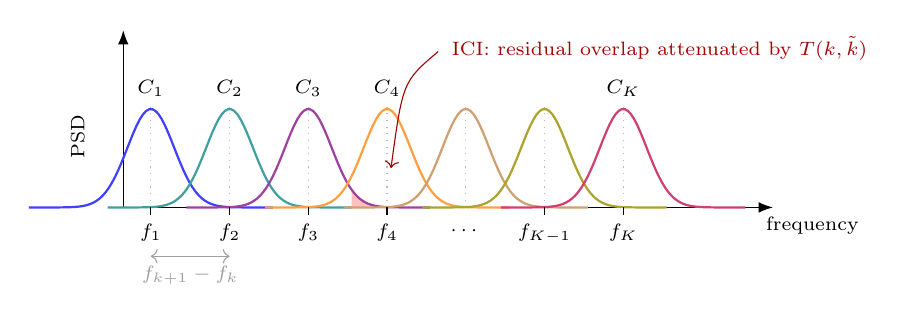
\begin{tikzpicture}[scale=1.0, font=\small]
  \def\sig{0.42}
  \def\amp{1.25}
  \draw[-{Latex[length=1.8mm]}] (-0.35,0) -- (7.9,0)
        node[below right=0pt and -6pt, font=\scriptsize] {frequency};
  \draw[-{Latex[length=1.8mm]}] (-0.35,0) -- (-0.35,2.25);
  \node[font=\scriptsize, rotate=90, anchor=south] at (-0.72,0.9) {PSD};
  \begin{scope}
    \clip (2.55,0) rectangle (3.45,2.0);
    \fill[red!25]
      plot[domain=2.5:3.5,samples=60] (\x,{\amp*exp(-((\x-2.0)/\sig)^2)})
      -- (3.5,0) -- (2.5,0) -- cycle;
  \end{scope}
  \foreach \i/\c in {0/blue,1/teal,2/violet,3/orange,4/brown,5/olive,6/purple}{
    \draw[\c!75, thick]
      plot[domain={\i-1.55}:{\i+1.55},samples=80]
      (\x,{\amp*exp(-((\x-\i)/\sig)^2)});
    \draw[gray!55, dotted] (\i,0) -- (\i,{\amp*1.02});
  }
  \foreach \i/\lab in {0/$f_1$,1/$f_2$,2/$f_3$,3/$f_4$,5/$f_{K-1}$,6/$f_K$}{
    \draw (\i,0) -- (\i,-0.09) node[below, font=\scriptsize] {\lab};
  }
  \node[font=\scriptsize] at (4,-0.3) {$\cdots$};
  \foreach \i/\lab in {0/$C_1$,1/$C_2$,2/$C_3$,3/$C_4$,6/$C_K$}{
    \node[font=\scriptsize, anchor=south] at (\i,{\amp*1.03}) {\lab};
  }
  \draw[<->, gray!75] (0,-0.62) -- (1,-0.62)
        node[midway, below, font=\scriptsize] {$f_{k+1}-f_{k}$};
  \node[font=\scriptsize, red!65!black, align=center, anchor=west]
        at (3.7,2.02) {ICI: residual overlap attenuated by $T(k,\tilde{k})$};
  \draw[->, red!65!black, thin] (3.65,1.98) .. controls (3.2,1.6) .. (3.05,0.5);
\end{tikzpicture}}
\caption{Non-orthogonal channel partition: adjacent channels overlap because of
spectral leakage, so a transmission on $\tilde{k}$ reaches a receiver tuned to
$k$ attenuated by $T(k,\tilde{k})$ rather than suppressed.}
\label{fig:channels}
\end{figure}

Propagation follows the Egli model~\cite{egli1957radio}. For users
$i,j\in\mathcal{N}^{n}$ with $i$ transmitting to $j$ on channel $k$, the
received SINR is
\begin{equation}
\begin{aligned}
\mathrm{SINR}^{\,n,n}_{\,i,j,k} &=
   \frac{PR^{\,n,n}_{\,i,j,k}}{I_{T} + I^{\,n}_{\,j,k}},\\
PR^{\,n,n}_{\,i,j,k} &= PT^{\,n}_{\,j,k} - PL^{\,n,n}_{\,i,j,k}
   - \chi^{\,n,n}_{\,i,j,k} - \psi^{\,n,n}_{\,i,j,k},
\end{aligned}
\label{eq:sinr}
\end{equation}
where $I_{T}$ is thermal noise, $I^{\,n}_{\,j,k}$ the aggregate interference
from $\mathcal{N}\setminus\mathcal{N}^{n}$, $PT$ the transmit power in dBW,
$PL$ the path loss, and $\chi,\psi$ the fading and shadowing terms. The Egli
path loss is
\begin{align}
PL^{\,n,n}_{\,i,j,k} =\;
 & 40\log_{10}\!\bigl(d^{\,n,n}_{\,i,j}\bigr)
 - 20\log_{10}\!\left(\frac{40}{f_{k}}\right) \nonumber\\
 & - 20\log_{10}\!\bigl(H^{n}_{T_{i}} H^{n}_{R_{j}}\bigr)
   - 10\log_{10}\!\bigl(G^{n}_{T_{i}} G^{n}_{R_{j}}\bigr)\;[\mathrm{dB}],
\label{eq:egli}
\end{align}
with $d$ the distance in meters, $f_{k}$ the carrier in MHz, $H_{T},H_{R}$ the
antenna heights and $G_{T},G_{R}$ the gains. Interference aggregates over all
other networks and their users,
\begin{equation}
I^{\,n}_{\,j,k} =\!\!\sum_{l\in\mathcal{N}\setminus\{n\}}
   \sum_{m=1}^{M^{l}}\! \phi^{\,n,l}_{\,j,m,k},
\qquad
\phi^{\,n,l}_{\,j,m,k} = PR^{\,n,l}_{\,j,m,k} - T(k,\tilde{k}),
\label{eq:interference}
\end{equation}
where $\tilde{k}$ is the channel occupied by the interferer. Equation
\eqref{eq:interference} is where non-orthogonality enters: for $\tilde{k}=k$ we
have $T=0$ and the interferer is felt at full strength, while for
$|k-\tilde{k}|\geq 1$ it is attenuated but not eliminated. The noise floor is
$I_{T}=10\log_{10}(k_{B}\,\mathrm{Temp}\,B)+10\log_{10}(\mathrm{NF})+30$~dBm,
equal to $-104.9$~dBm at room temperature with $B=2$~MHz and a $6$~dB noise
figure.

\emph{Scenario generation and the network manager.} The number of networks $N$
is sampled uniformly, and each $M^{n}$ is drawn uniformly from
$\{1,\dots,M_{\max}\}$; users scatter around their network center by a
bivariate Gaussian with covariance
$\mathrm{diag}(50^{2},50^{2})~\mathrm{m}^{2}$. Centers are placed
sequentially: the first uniformly over a square whose extent grows with $N$,
and every subsequent center attached to a randomly chosen existing center at a
random radius $r\sim U[x_{1},x_{2}]$ and angle $\theta\sim
U[0,2\pi]$.\footnote{The reference implementation released
with~\cite{cohen2024carlton} draws $r$ and $\theta$ with an integer-valued
sampler, restricting $\theta$ to six discrete angles. We corrected this in both
our framework and the reproduced centralized baseline, so that all methods are
trained and evaluated on identically distributed topologies.} This produces
clustered, partially overlapping deployments rather than a uniform scatter,
which is what makes the interference graph non-trivial. Within each network the
user minimizing the total distance to all others is designated the
\emph{network manager}, mirroring the centralized-unit role in 5G local
networks: it gathers the per-user reports over a dedicated control channel,
selects the channel, and disseminates the decision.
Fig.~\ref{fig:scenario} shows a representative instance. Decisions are
sequential: each network is assigned a serial number fixing its turn, which
emulates propagation and processing delays and prevents simultaneous
conflicting decisions. The horizon is $T\,N$ steps, so every network receives
exactly $T$ decision points regardless of $N$.

%------------------------------------------------------------------------------
\subsection{The Objective}
\label{subsec:model_objective}
%------------------------------------------------------------------------------

Let $c^{n}\in\mathcal{K}$ denote the channel of $\mathcal{N}^{n}$. Averaging
\eqref{eq:sinr} over the messages a user receives from the other $M^{n}-1$
users, and then over users, yields the network-level quantity
$\overline{\mathrm{SINR}}^{\,n}_{\,c^{n}}$. The allocation goal is to maximize
the mean network SINR subject to a target QoS level for \emph{every}
participating network,
\begin{equation}
\max_{\{c^{n}\}} \frac{1}{N}\sum_{n=1}^{N}
      \overline{\mathrm{SINR}}^{\,n}_{\,c^{n}}
\quad\text{s.t.}\quad \overline{\mathrm{SINR}}^{\,n}_{\,c^{n}}
      \geq \mathrm{SINR}^{*},\;\; \forall n .
\label{eq:objective}
\end{equation}
The constraint is essential: maximizing the average alone admits solutions in
which a few well-placed networks capture most of the spectrum while others are
starved.

Solving \eqref{eq:objective} directly would require each manager to collect
real-valued SINR measurements from all of its users on all $K$ channels, which
is prohibitive for large networks and battery-limited terminals. Each user
therefore reports a single bit per channel,
$\mathrm{BSINR}^{\,n}_{\,j,k}=\mathbf{1}(\mathrm{SINR}^{\,n}_{\,j,k} >
\mathrm{SINR}_{T})$, and the manager averages the resulting $M^{n}\times K$
matrix along the user axis to obtain the \emph{quality vector}
\begin{equation}
\mathrm{QV}^{\,n}_{k}
 = \frac{1}{M^{n}}\sum_{j=1}^{M^{n}} \mathrm{BSINR}^{\,n}_{\,j,k}
 \;\in[0,1] .
\label{eq:qv}
\end{equation}
Entry $\mathrm{QV}^{\,n}_{k}$ is the fraction of users of $\mathcal{N}^{n}$
that would meet the QoS target on channel $k$; averaging removes the dependence
on network size. Under this communication constraint the objective becomes
$\max_{\{c^{n}\}} \frac{1}{N}\sum_{n} \overline{\mathrm{BSINR}}^{\,n}_{\,c^{n}}$
subject to the same per-network floor. The quality vector is the only
environmental information available to the agent---and, in the centralized
paradigm, the quantity that must be shipped to the global replay memory.
Measuring SINR across all channels presupposes wideband sensing, which modern
software-defined radio front ends make practical~\cite{arjoune2019comprehensive}.

%------------------------------------------------------------------------------
\subsection{The Federated Learning Problem}
\label{subsec:model_federated}
%------------------------------------------------------------------------------

Each network manager is a computing node that privately holds all data
generated by its own network: the per-user BSINR reports, the quality vectors
$\mathrm{QV}^{n}(t)$, the channels it selected, and the rewards it received.
Identifying the manager of $\mathcal{N}^{n}$ with federated client $n$
therefore requires no additional infrastructure assumption---it merely refrains
from exporting data the manager already possesses. Writing $F_{n}(w)$ for the
expected temporal-difference loss incurred by parameters $w$ on the transitions
stored at client $n$, and $n_{k}$ for the number of samples it holds, learning
becomes the federated problem
\begin{equation}
\min_{w}\; F(w) = \sum_{k=1}^{N} \frac{n_{k}}{\sum_{j} n_{j}}\, F_{k}(w),
\label{eq:fed_objective}
\end{equation}
whereas CTDE training minimizes a single empirical loss over the union of all
clients' transitions. The two coincide only when the local distributions are
identical, which here they demonstrably are not.

Three structural properties make the local objectives genuinely heterogeneous,
and all three are visible in Fig.~\ref{fig:scenario}. First, $M^{n}$ varies
over an order of magnitude across networks, and since \eqref{eq:qv} averages
over $M^{n}$ users, quality vectors of small and large networks differ in
granularity and noise. Second, the number of networks within the neighbor
threshold $\Gamma$ differs across agents, so agents at the center of a cluster
face dense interference while peripheral agents see an almost empty spectrum.
Third, because a network's observation depends on the channels currently
occupied by its neighbors, each client's distribution is continuously reshaped
by the concurrent policy updates of the others, making the local objectives
both non-stationary and mutually coupled.

\begin{figure}[!t]
\centering
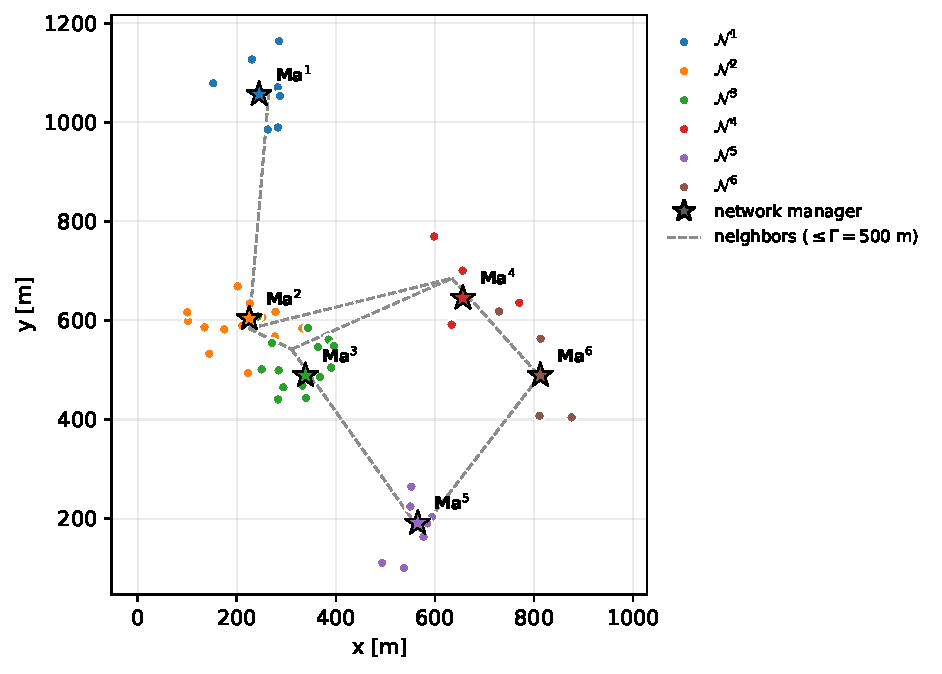
\includegraphics[width=0.86\columnwidth]{scenario_illustration.pdf}
\caption{Representative six-network scenario produced by our simulator. Dots
are users colored by network, stars mark the network managers, and dashed lines
connect networks within the neighbor threshold $\Gamma=500$~m. The asymmetry in
user counts and neighborhood sizes is the structural origin of the non-IID
client experience.}
\label{fig:scenario}
\end{figure}

%==============================================================================
\section{\texorpdfstring{The \OURS{} Algorithm}{The CARLTON FL Algorithm}}
\label{sec:method}
%==============================================================================

%------------------------------------------------------------------------------
\subsection{Background: Value-Based DRL without a Target Network}
\label{subsec:method_drl}
%------------------------------------------------------------------------------

Each network manager is an autonomous agent that observes its environment,
selects a channel, and receives a scalar reward. We use value-based
reinforcement learning, in which the agent estimates
$Q_{\pi}(s,a)=\mathbb{E}_{\pi}[\sum_{i\geq0}\gamma^{i} r(t{+}i{+}1)\mid
S(t)=s,A(t)=a]$ with discount $\gamma\in(0,1)$, approximates it by a network
$Q(s,a;w)$, and fits it by minimizing the temporal-difference (TD)
error~\cite{sutton2018reinforcement}.

Standard deep $Q$-networks form the bootstrapped target with a delayed copy
$w^{-}$ of the parameters. Such a target network is a poor fit for a federated
system, because the delayed copy is a second piece of state that would have to
be either synchronized with the aggregation schedule or kept private and thus
inconsistent across clients. We therefore build the learner on
DeepMellow~\cite{kim2019deepmellow}, which replaces the hard maximum by the
mellowmax operator~\cite{asadi2017alternative},
\begin{equation}
\mathrm{mm}_{\omega}\bigl(Q(s,\cdot\,;w)\bigr)
 = \frac{1}{\omega}\,
   \log\!\left(\frac{1}{K}\sum_{k=1}^{K} e^{\,\omega\, Q(s,k;w)}\right),
\label{eq:mellowmax}
\end{equation}
a smooth surrogate recovering the mean as $\omega\to 0$ and the maximum as
$\omega\to\infty$. Because mellowmax is a non-expansion and softens the
maximization bias that motivates the target network in the first place, stable
learning is attained \emph{without} a delayed copy---which is precisely what
makes the client state in our framework a single parameter vector. The target
of client $n$ is therefore
\begin{equation}
Y^{n}(t) = r^{n}(t+1)
  + \gamma\,\bigl(1 - d(t+1)\bigr)\,
    \mathrm{mm}_{\omega}\bigl(Q(s^{n}(t+1),\cdot\,;w)\bigr),
\label{eq:target}
\end{equation}
computed from the online parameters under a stop-gradient, with $d$ the
terminal indicator. With $e^{n}(t)=Y^{n}(t)-Q(s^{n}(t),a^{n}(t);w)$, the
per-sample loss is the Huber loss $L_{\delta}(e)$, whose linear tail limits the
influence of the rare large TD errors that a non-stationary multi-agent
environment inevitably produces. The value network is a three-layer residual
multilayer perceptron with $128$ units per layer, Leaky-ReLU activations of
slope $0.2$, an identity output layer of width $K$, and \texttt{PyTorch}'s
default Kaiming-uniform initialization~\cite{he2015delving}; it holds
$d_{w}=36{,}234$ parameters for $K=10$, and is common to all methods compared
in Section~\ref{sec:experiments}.

%------------------------------------------------------------------------------
\subsection{Observation Space, Action Space, and Exploration}
\label{subsec:method_state}
%------------------------------------------------------------------------------

The state concatenates the quality vector \eqref{eq:qv} with a binary encoding
of the channel currently occupied,
\begin{equation}
s^{n}(t) = \bigl[\mathrm{CBR}^{n}(t); \mathrm{QV}^{n}(t)\bigr]
  \in \mathbb{R}^{\,B+K},\;\; B = \lfloor \log_{2}K \rfloor + 1 ,
\label{eq:state}
\end{equation}
where $\mathrm{CBR}^{n}(t)\in\{0,1\}^{B}$ is the channel binary representation
of the previous allocation; including it is what allows the agent to
distinguish ``stay'' from ``switch'' and hence to learn the spectrum-mobility
trade-off. The action space is the channel set $\mathcal{K}$, so the output
layer has one value per channel.

Two mechanisms shape action selection. First, channels on which no user would
meet the QoS target are removed by invalid-action masking,
$\widetilde{Q}(s^{n},k;w) = -\infty$ if $\mathrm{QV}^{\,n}_{k}=0$ and
$Q(s^{n},k;w)$ otherwise; in the degenerate case
$\mathrm{QV}^{n}=\mathbf{0}$ no decision is taken and the current channel is
retained. Masking prevents wasted exploration on provably unusable channels and
reduces collisions. Second, exploration follows a Boltzmann policy over the
masked values,
\begin{equation}
\Pr\bigl(a^{n}(t)=k \mid s^{n}(t)\bigr)
 = \frac{e^{\,\beta \widetilde{Q}(s^{n}(t),k;w)}}
        {\sum_{k'\in\mathcal{K}} e^{\,\beta \widetilde{Q}(s^{n}(t),k';w)}},
\label{eq:explore}
\end{equation}
sampled with probability $\epsilon_{b}$ and replaced by the greedy choice
otherwise. We anneal $\epsilon_{b}$ linearly from $0.5$ to $0.01$ over the first
half of training and hold it fixed thereafter. Note that $\epsilon_{b}$ is a
global schedule indexed by the communication round: all clients in a round
explore at the same rate, which keeps the cohort's data collection
statistically comparable.

%------------------------------------------------------------------------------
\subsection{Reward Design and the Locality of the Learning Signal}
\label{subsec:method_reward}
%------------------------------------------------------------------------------

The reward must express two competing goals: occupy a high-quality channel, and
stop moving once a good allocation has been found. The personal component
$r_{p}$ of Algorithm~\ref{alg:rp} does both. It grants a large fixed reward
$r_{\mathrm{desired}}$ when the fraction of satisfied users on the chosen
channel exceeds a threshold $\zeta$; otherwise it returns the rank of the
chosen channel among all $K$ channels, mapped to $[-1,1]$, so that selecting
the best available channel is rewarded even when no channel is outright good. A
multiplicative bonus $c_{1}>1$ is applied when the agent keeps its previous
channel, penalizing needless spectrum mobility. With $\zeta=0.9$,
$r_{\mathrm{desired}}=4$, $c_{1}=1.1$ and $T=20$ decision points per episode,
the maximum attainable accumulated reward is
$T\,c_{1}r_{\mathrm{desired}}=88$, which we use in
Section~\ref{sec:experiments} as an absolute reference.

\begin{algorithm}[!t]
\caption{Personal reward $r_{p}$ of network $\mathcal{N}^{n}$}
\label{alg:rp}
\begin{algorithmic}[1]
\Require $\mathrm{QV}^{n}(t)$, actions $a^{n}(t)$, $a^{n}(t-1)$
\Ensure  $r_{p}$
\State $v \gets \mathrm{QV}^{\,n}_{a^{n}(t)}(t)$
\If{$v \geq \zeta$}
  \State $r_{p} \gets r_{\mathrm{desired}}$
\Else
  \State $\mathrm{SQV}^{n} \gets \mathrm{sort}\bigl(\mathrm{QV}^{n}(t)\bigr)$;\;
         $i \gets 0$
  \While{$i \leq K$ \textbf{and} $v \geq \mathrm{SQV}^{n}_{i}$}
    \State $i \gets i+1$
  \EndWhile
  \State $r_{p} \gets 2\left(i/K - 0.5\right)$
       \Comment{rank of the chosen channel}
\EndIf
\If{$a^{n}(t) = a^{n}(t-1)$ \textbf{and} $r_{p} > 0$}
  \State $r_{p} \gets c_{1}\, r_{p}$ \Comment{stability bonus}
\EndIf
\end{algorithmic}
\end{algorithm}

A social-welfare component $r_{sw}$ makes each agent accountable for the
externalities it imposes on its neighbors. With the interference neighborhood
$\mathcal{B}^{n}=\{m\neq n : \lVert \mu^{m}-\mu^{n}\rVert_{2}\leq \Gamma\}$,
it is the mean personal reward collected by those neighbors between two
consecutive decisions of network $n$ (zero if $\mathcal{B}^{n}=\emptyset$), and
the total reward is the convex combination
\begin{equation}
r = \rho\, r_{p} + (1-\rho)\, r_{sw},
\label{eq:reward}
\end{equation}
with personal-reward fraction $\rho\in[0,1]$ trading self-interest against
cooperation.

This construction deserves attention in a federated context, because it is the
one place where an agent's reward depends on quantities computed by others:
evaluating $r_{sw}$ requires network $n$ to learn the personal rewards obtained
by its neighbors, an exchange of information during \emph{training} that is
modest but real. Setting $\rho = 1$ removes the term altogether and makes the
learning signal strictly local---an agent then needs nothing beyond its own
quality vector and action history. We adopt $\rho = 1$ in \OURS{} for exactly
this reason, and retain $\rho = 0.7$ for the centralized baseline, which
already assumes a coordinator pooling all trajectories and for which the social
term is therefore free. Our framework thus operates under a \emph{stricter}
information constraint than the baseline it is compared against, making the
comparison conservative rather than favorable;
Section~\ref{sec:experiments} reports a control experiment isolating $\rho$.

%------------------------------------------------------------------------------
\subsection{Federated Training Procedure}
\label{subsec:method_loop}
%------------------------------------------------------------------------------

Training proceeds over $B$ communication rounds, summarized in
Algorithm~\ref{alg:frl}. In round $t$ the server \textbf{broadcasts} $w^{t}$ to
all participating clients. A scenario with $N_{t}$ networks is then generated
and played for $T\,N_{t}$ steps (\textbf{interaction}), so that every client
obtains exactly $T$ decision points and appends the corresponding transitions
to its own persistent memory $\mathcal{D}^{n}$. Each client then performs $E$
gradient steps on mini-batches of size $b_{z}$ drawn from $\mathcal{D}^{n}$
alone (\textbf{local update}); clients holding fewer than $b_{z}$ transitions
skip the update and return the broadcast model unchanged, which occurs only in
the earliest rounds. Finally the clients upload $w^{t,E}_{n}$ and the server
\textbf{aggregates} them into $w^{t+1}$.

Two features distinguish this loop from textbook federated learning. First, the
dataset is not fixed: clients \emph{generate} their own data with the policy
they are currently learning, so $\mathcal{D}^{n}$ grows and its distribution
shifts as training progresses. Persistence is what makes this workable---a
buffer retained across rounds preserves experience gathered under earlier
policies and topologies, which both stabilizes the TD targets and prevents a
client from overfitting the single episode it has just played. Second, the
cohort is redrawn each round, since $N_{t}$ is resampled and a fresh topology
generated. This is structurally identical to partial client participation, and
it has the useful side effect that the global model is never allowed to
specialize to one deployment geometry.

\emph{Local objective.} Let $F_{n}(w) = \mathbb{E}_{(s,a,r,s')\sim
\mathcal{D}^{n}}[L_{\delta}(e(s,a,r,s';w))]$ be the expected TD loss at client
$n$. In \FedAvg{} each client simply applies $E$ stochastic gradient steps to
$F_{n}$. This is the natural baseline, and when $E$ is small it is a good one;
but the whole point of many local steps is to reduce the number of
communication rounds, and as $E$ grows each client converges toward the
minimizer of its \emph{own} objective. Under the heterogeneity of
Section~\ref{subsec:model_federated} those minimizers are far apart and their
average need not be good for any of them---the client-drift phenomenon.
\FedProx{}~\cite{li2020fedprox} addresses it by replacing the local objective
with the proximal surrogate
\begin{equation}
h_{n}\bigl(w; w^{t}\bigr) = F_{n}(w)
  + \frac{\mu}{2}\,\bigl\lVert w - w^{t} \bigr\rVert_{2}^{2},
\label{eq:prox_local}
\end{equation}
whose gradient adds a restoring force $\mu(w-w^{t})$ toward the broadcast model
at every local step. The penalty does not forbid local progress; it bounds how
far a client may travel from the consensus point within a round, which is
precisely the quantity that determines whether averaging is meaningful. Thus
$\mu$ interpolates between two failure modes: $\mu=0$ recovers \FedAvg{}
exactly---a property we assert as a numerical regression test on the
implementation---while excessively large $\mu$ freezes the clients at $w^{t}$.

The proximal term is a particularly natural fit here. In supervised federated
learning the anchor $w^{t}$ is merely a consensus point; in value-based
reinforcement learning it is additionally the parameter vector that generated
the bootstrapped targets \eqref{eq:target} at the start of the round, so
penalizing displacement from $w^{t}$ also limits the extent to which each
client chases a target it is itself moving---an off-policy instability that is
independent of federation but amplified by long local phases.

%------------------------------------------------------------------------------
\subsection{Aggregation and Why Federation Helps}
\label{subsec:method_agg}
%------------------------------------------------------------------------------

The server combines the uploaded models by weighted averaging,
$w^{t+1} = \sum_{n \in \mathcal{C}_{t}} (n_{k}/\sum_{j\in\mathcal{C}_{t}}
n_{j})\, w^{t,E}_{n}$, where $\mathcal{C}_{t}$ is the cohort of round $t$ and
$n_{k}$ the number of transitions contributed by client $k$. Because the
horizon is fixed at $T\,N_{t}$ steps, every client collects exactly $T$ new
transitions per round, so the weights are uniform and aggregation reduces to
the plain mean. This is a consequence of the round-robin turn structure of the
environment, not an assumption. Aggregation is performed independently per
parameter tensor and is therefore agnostic to the architecture.

Since all clients start the round from the same $w^{t}$, it is convenient to
write the update in terms of the local displacements
$\Delta_{n}^{t} = w^{t,E}_{n} - w^{t}$, giving
$w^{t+1} = w^{t} + |\mathcal{C}_{t}|^{-1}\sum_{n} \Delta_{n}^{t}$. In this form
the mechanism by which federation helps is explicit: the global step is the
mean of $|\mathcal{C}_{t}|$ displacements computed from independently sampled
topologies and independently sampled mini-batches. Components of
$\Delta^{t}_{n}$ reflecting a client's idiosyncratic interference neighborhood
are attenuated by averaging, while components shared across clients survive.
Periodic averaging thus acts as a variance-reduction mechanism on top of, and
orthogonal to, mini-batch averaging---which is why we expect, and in
Section~\ref{sec:experiments} observe, federated training not merely to
tolerate the loss of centralized experience but to benefit from its absence.

\begin{algorithm}[!t]
\caption{\OURS{} training procedure}
\label{alg:frl}
\begin{algorithmic}[1]
\Require Rounds $B$, local steps $E$, proximal weight $\mu$, batch size
         $b_{z}$, buffer capacity $S_{z}$, schedule $\{\epsilon_{b}(t)\}$
\Ensure  Global policy parameters $w^{*}$
\State Server initializes $w^{0}$; each client $n$ initializes an empty
       persistent $\mathcal{D}^{n}$ of capacity $S_{z}$
\For{$t = 0,\dots,B-1$}
  \State Sample $N_{t}$, generate a scenario, let $\mathcal{C}_{t}$ be the
         participating clients
  \State \textbf{Broadcast:} $w^{t,0}_{n} \gets w^{t}$,\;
         $\forall n \in \mathcal{C}_{t}$
  \For{$\tau = 1,\dots,T$}\Comment{interaction phase}
    \For{$n \in \mathcal{C}_{t}$ \textbf{in turn order}}
      \State Collect BSINR reports; form $\mathrm{QV}^{n}$ by \eqref{eq:qv} and
             $s^{n}(\tau)$ by \eqref{eq:state}
      \State Select $a^{n}(\tau)$ by \eqref{eq:explore} with $\epsilon_{b}(t)$;
             observe $r^{n}$, $s^{n}(\tau{+}1)$
      \State $\mathcal{D}^{n} \gets \mathcal{D}^{n} \cup
             \{(s^{n}(\tau),a^{n}(\tau),r^{n},s^{n}(\tau{+}1))\}$
    \EndFor
  \EndFor
  \For{$n \in \mathcal{C}_{t}$}\Comment{local update, in parallel}
    \If{$|\mathcal{D}^{n}| \geq b_{z}$}
      \For{$e = 1,\dots,E$}
        \State Sample a mini-batch of size $b_{z}$ from $\mathcal{D}^{n}$
        \State $w^{t,e}_{n} \gets w^{t,e-1}_{n} - \eta\,\nabla
               \bigl[\widehat{F}_{n} + \tfrac{\mu}{2}
               \lVert w^{t,e-1}_{n} - w^{t}\rVert^{2}\bigr]$
      \EndFor
    \Else
      \State $w^{t,E}_{n} \gets w^{t}$
    \EndIf
    \State Upload $w^{t,E}_{n}$
  \EndFor
  \State \textbf{Aggregate:} $w^{t+1} \gets
         \frac{1}{|\mathcal{C}_{t}|}\sum_{n \in \mathcal{C}_{t}} w^{t,E}_{n}$
\EndFor
\State \Return $w^{*} \gets w^{B}$
\end{algorithmic}
\end{algorithm}

%------------------------------------------------------------------------------
\subsection{Cost, Execution, and Privacy}
\label{subsec:method_cost}
%------------------------------------------------------------------------------

It is worth quantifying what the change of paradigm costs and saves, since the
answer is not uniformly favorable. \emph{Downlink} is unchanged: both paradigms
broadcast the model to every manager before each episode. \emph{Uplink} differs
in kind. CTDE uploads $T$ raw transitions of $2(B+K)+3$ scalars each, about
$2.5$~kB per client per round, whereas \OURS{} uploads $d_{w}=36{,}234$
parameters, about $145$~kB---roughly $58\times$ more for a model this compact.
We state this plainly: federated training is not, here, a bandwidth
optimization. What it buys is that the payload is \emph{fixed in size and
content-independent}: it does not grow with the number of users $M^{n}$, with
episode length, or with buffer retention, and it carries no measurement
attributable to a specific user. Where uplink is binding, the standard remedies
apply unmodified---$8$-bit quantization divides the cost fourfold, and
aggregating every $R$ rounds divides it by $R$. \emph{Computation} moves in the
opposite direction: instead of all gradient steps running on one node whose
load grows with the deployment, each client performs $E$ steps on its own
hardware concurrently, at cost $O(E\,b_{z}\,d_{w})$ independent of $N_{t}$, and
a client that drops out simply does not contribute to the average, whereas the
loss of a central learner halts CTDE training entirely.

Once training terminates, $w^{*}$ is distributed to the managers and the server
is discarded. Execution is fully distributed and message-free: at each decision
instant a manager collects the BSINR reports of its own users, forms
$\mathrm{QV}^{n}$, applies the mask, and selects
$\arg\max_{k}\widetilde{Q}(s^{n},k;w^{*})$ with a single forward pass. The
federated construction thus changes the training phase only, leaving intact the
deployment properties that motivate distributed DCA in the first place.

Regarding privacy, our claim is precise and deliberately limited. What is
eliminated is the export of raw sensing data---the per-user BSINR reports, the
quality vectors, the occupied-channel sequence, and the rewards---which are
exactly the quantities from which an observer of a global replay memory could
reconstruct a network's spatial situation, load, and traffic pattern. What
remains exposed is the parameter update $\Delta^{t}_{n}$, and model deltas are
known to leak information about the data that produced
them~\cite{kairouz2021advances}. We therefore do not claim formal privacy, but
note that \OURS{} is compatible without algorithmic modification with the
standard defenses: secure aggregation reveals only the sum to the server, and
differentially private updates follow from clipping $\Delta^{t}_{n}$ and adding
calibrated noise. Quantifying the resulting privacy--utility trade-off is left
to future work.

%==============================================================================
\section{Experiments and Discussion}
\label{sec:experiments}
%==============================================================================

In this section we present the experimental study of \OURS{}. We begin with the
simulation environment and the evaluation protocol in
Subsection~\ref{subsec:exp_setup}, and define in
Subsection~\ref{subsec:exp_metrics} the physical performance measures used
throughout, which are the ones introduced for the centralized state of the art
in~\cite{cohen2024carlton}. Subsection~\ref{subsec:exp_reward} analyzes the
training behavior of \OURS{}, and Subsection~\ref{subsec:exp_paper} provides a
performance comparison against \CARLTON{} and the alternative algorithms
evaluated in~\cite{cohen2024carlton}.

%------------------------------------------------------------------------------
\subsection{Simulation Environment and Evaluation Protocol}
\label{subsec:exp_setup}
%------------------------------------------------------------------------------

The simulation environment follows Section~\ref{subsec:model_system}: a total
band split into $K=10$ overlapping channels with carriers spaced $2$~MHz apart
over $208$--$226$~MHz, Egli propagation, the spectral attenuation schedule of
Section~\ref{subsec:model_system}, and a thermal noise floor of
$I_{T}=-104.9$~dBm. In every scenario instance the number of networks $N$ is
drawn at random, each network serves $M^{n}\sim U\{1,\dots,15\}$ users
scattered around its center by a bivariate Gaussian with covariance
$\mathrm{diag}(50^{2},50^{2})~\mathrm{m}^{2}$, and centers are placed
sequentially at a random radius $r\sim U[50,500]$~m and angle $\theta\sim
U[0,2\pi]$ from a previously placed center. Each network is managed by the user
minimizing the total distance to all others, and every network receives exactly
$T=20$ decision points, so the scenario horizon is $T\,N$ steps.
Fig.~\ref{fig:scenario} illustrates a representative instance.

Training scenarios are restricted to $N\leq 7$ networks, as
in~\cite{cohen2024carlton}; scenarios with $N>7$ are therefore never seen
during training and are used to probe generalization. Every run comprises
$B=1000$ rounds (episodes for the centralized baselines) followed by $100$
frozen-weight inference episodes, with $\epsilon_{b}$ annealed from $0.5$ to
$0.01$ over the first half of training. The value network is the
$36{,}234$-parameter residual MLP of Section~\ref{subsec:method_drl}, and all
remaining hyperparameters follow Table~II of~\cite{cohen2024carlton}. We report
four methods over $30$ independent seeds each:

\begin{itemize}
\item \emph{\CARLTON{}}: centralized CTDE baseline with a shared global replay
  memory and $\rho=0.7$;
\item \emph{TF CTDE}: TensorFlow centralized baseline under the same reward
  ($\rho=0.7$);
\item \FedAvg{}: federated training with $E=10$ local steps and $\mu=0$;
\item \FedProx{}: the same with proximal weight $\mu=0.01$.
\end{itemize}

The pair $(E,\mu)=(10,0.01)$ is the outcome of a prior sweep over
$E\in\{1,5,10,20\}$ and $\mu\in\{0,0.001,0.01,0.1\}$. Federated clients use
personal reward only ($\rho=1$) and never observe a neighbor's reward, whereas
the centralized baselines retain the social term ($\rho=0.7$); the federated
setting is thus the stricter one from an information standpoint. Following the
protocol of~\cite{cohen2024carlton}, trained policies are finally evaluated on
$30$ games for each $N\in\{2,\dots,15\}$, i.e., $420$ games per algorithm.

%------------------------------------------------------------------------------
\subsection{Performance Metrics}
\label{subsec:exp_metrics}
%------------------------------------------------------------------------------

We adopt the physical performance measures defined
in~\cite{cohen2024carlton}, so that our results are directly comparable with
the reported behavior of the centralized state of the art. Let $c^{n}(t)$
denote the channel occupied by network $\mathcal{N}^{n}$ at step $t$, and
recall the quality vector $\mathrm{QV}^{n}$ of~\eqref{eq:qv}. At the end of a
scenario the \emph{channel quality} (CQ) vector collects the quality each
network actually experiences on the channel it settled on,
\begin{equation}
\begin{gathered}
\mathrm{CQ}=\left[\mathrm{QV}^{1}_{c^{1}(T)}(T),\dots,
\mathrm{QV}^{N}_{c^{N}(T)}(T)\right],\\
\overline{\mathrm{CQ}}=\mathbb{E}[\mathrm{CQ}],\qquad
\min\nolimits_{\mathrm{CQ}}=\min(\mathrm{CQ}).
\end{gathered}
\label{eq:cq}
\end{equation}
The mean $\overline{\mathrm{CQ}}$ measures aggregate spectral health, while
$\min_{\mathrm{CQ}}$ measures fairness: it is the quality of the
worst-served network, and it is the term that a purely self-interested
allocation tends to sacrifice. Their average,
$\mathbb{E}[(\mathrm{CQ}+\min_{\mathrm{CQ}})/2]$, is the composite reported in
Figs.~13 and~15 of~\cite{cohen2024carlton} and is our primary metric.

Spectrum mobility is captured by the average number of channel changes until
convergence per network (ANCC), normalized into a score
\begin{equation}
\mathrm{ANCCS}=1-\frac{\mathrm{ANCC}}{T},
\label{eq:anccs}
\end{equation}
and by the convergence time (CT), defined as the step of the last channel
change performed by any network in the scenario, with score
\begin{equation}
\mathrm{CTS}=1-\frac{\mathrm{CT}}{T\cdot N}.
\label{eq:cts}
\end{equation}
Both matter operationally: each channel change costs signaling and a brief
service interruption, and a slow-converging allocation is useless in a band
whose occupancy changes on the same timescale.

The third measure is the spectrum efficiency score (SES), which quantifies how
much clean spectrum the converged allocation leaves behind for a network that
might join later,
\begin{equation}
\mathrm{SES}=\mathbb{E}[\Psi]=\frac{1}{N}\sum_{n=1}^{N}\Psi^{n},\quad
\Psi^{n}=\Big(\sum_{k=1}^{K}\big(\mathrm{QV}^{n}_{k}(T)\big)^{2}\Big)^{0.5}
\big/K^{0.5}.
\label{eq:ses}
\end{equation}
A high SES indicates that the incumbents converged to a solution that distorts
few of the remaining channels.

Finally, these quantities are combined into the linear weighted score
\begin{equation}
\mathrm{WS}=w_{1}\overline{\mathrm{CQ}}+w_{2}\mathrm{ANCCS}
+w_{3}\mathrm{CTS}+w_{4}\mathrm{SES},
\label{eq:ws}
\end{equation}
with $(w_{1},w_{2},w_{3},w_{4})=(0.4,0.1,0.4,0.1)$ as
in~\cite{cohen2024carlton}. The larger weights are placed on
$\overline{\mathrm{CQ}}$ and CTS because sustained channel quality determines
whether the QoS-SINR constraint of~\eqref{eq:objective} is met at all, and fast
convergence determines whether the allocation is still valid by the time it is
reached; ANCCS and SES receive smaller weights since reduced mobility and
residual spectrum cleanliness are desirable but secondary to meeting QoS
quickly.

%------------------------------------------------------------------------------
\subsection{\texorpdfstring{\OURS{}'s Training Results}{CARLTON FL's Training Results}}
\label{subsec:exp_reward}
%------------------------------------------------------------------------------

Beyond the DeepMellow training reward, we track the physical rate that the
learned allocation actually delivers. For each saved global checkpoint we
freeze the weights, play a fixed set of in-sample scenarios, and convert the
SINR each network achieves on its final channel into a Shannon rate
\begin{equation}
R^{n}=B\log_{2}\!\bigl(1+\mathrm{SINR}^{n}\bigr),\qquad B=2~\mathrm{MHz},
\label{eq:shannon}
\end{equation}
averaged over the users of network $\mathcal{N}^{n}$.
Fig.~\ref{fig:throughput} reports the network-mean rate in Mbps as a function
of the training round for \FedAvg{} and \FedProx{} (mean $\pm$ std over three
seeds). Both curves rise sharply in the first few hundred rounds and then
saturate near their final operating point, confirming that the federated
policies translate the improving value estimates into higher delivered
throughput---not merely into a higher surrogate reward.

\begin{figure}[!t]
\centering
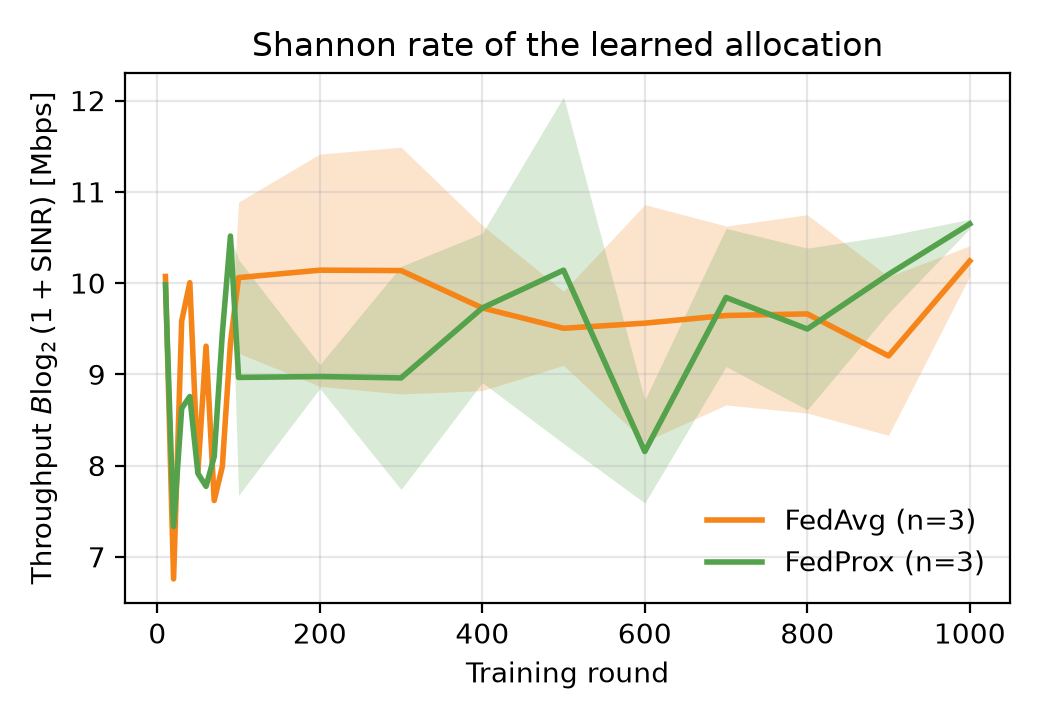
\includegraphics[width=\columnwidth]{campaign/throughput_vs_round.png}
\caption{Shannon throughput
$B\log_{2}(1+\mathrm{SINR})$ versus training round for \FedAvg{} and
\FedProx{} (mean $\pm$ std over $3$ seeds, identical evaluation scenarios at
every checkpoint). Channel bandwidth $B=2$~MHz.}
\label{fig:throughput}
\end{figure}

The number of local steps $E$ between aggregations is the main free parameter
of Algorithm~\ref{alg:frl}. Fig.~\ref{fig:e_sweep} sweeps
$E\in\{10,20,40,80,160\}$ for \FedProx{} ($\mu=0.01$) and scores the final
global model of each arm on inference reward, composite channel quality, and
Shannon throughput. All three panels peak at $E=10$, which is therefore the
operating point used throughout the rest of the paper; longer local phases
($E\geq 20$) lose a measurable fraction of quality, consistent with the
bias--variance trade-off that \FedProx{} is designed to regularize.

\begin{figure}[!t]
\centering
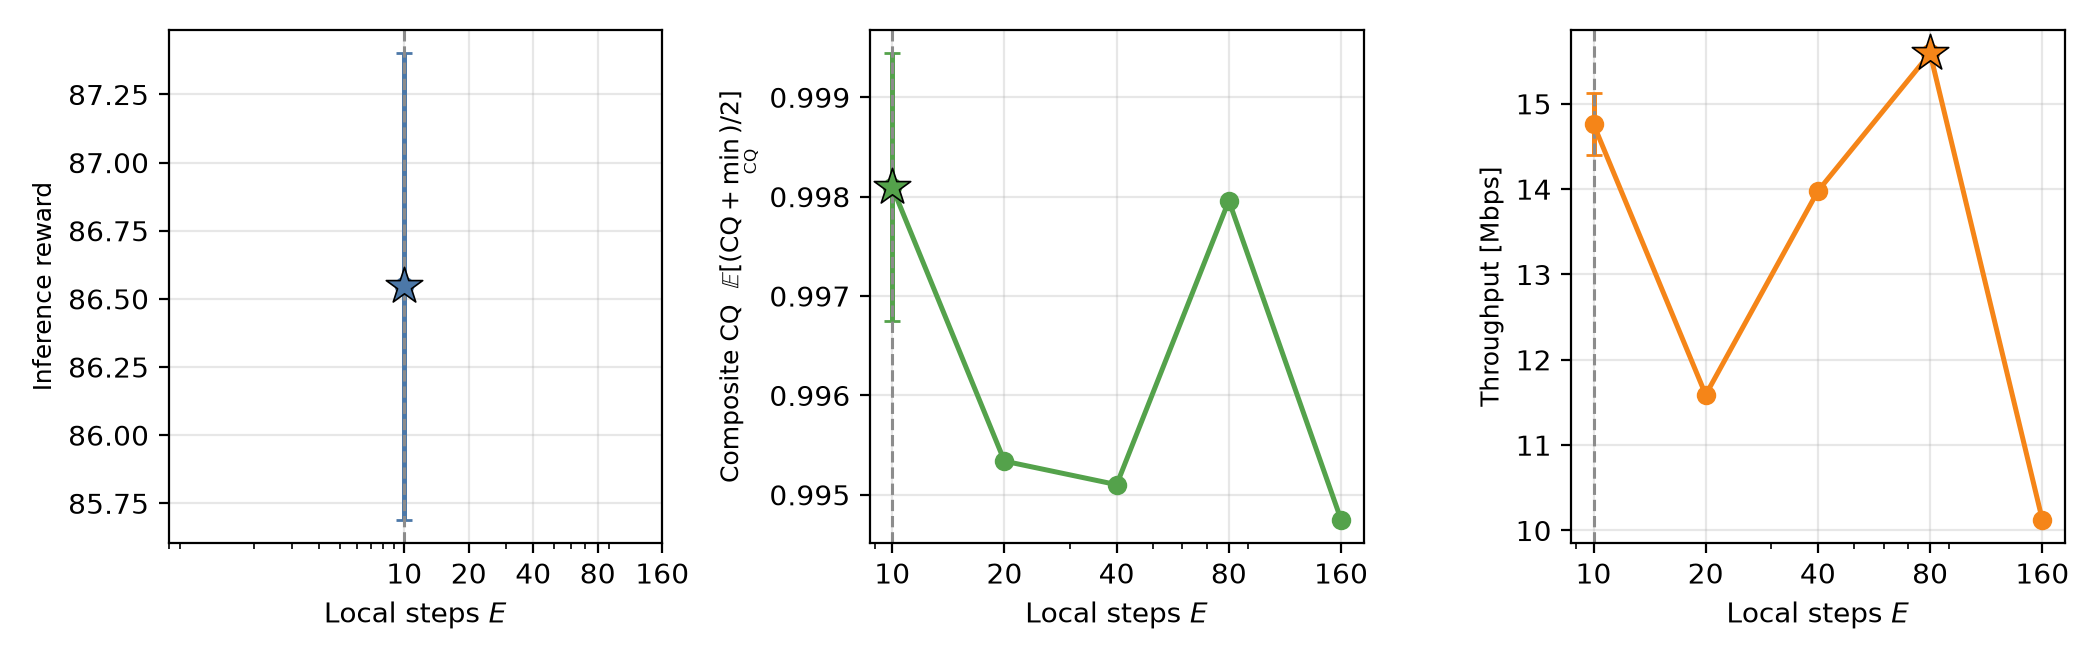
\includegraphics[width=\columnwidth]{campaign/e_sweep.png}
\caption{Sensitivity of \FedProx{} ($\mu=0.01$) to the number of local steps
$E$. Left: post-training inference reward. Middle: composite channel quality
$\mathbb{E}[(\mathrm{CQ}+\min_{\mathrm{CQ}})/2]$. Right: Shannon throughput
[Mbps]. The dashed line marks the chosen operating point $E=10$; the star
marks the empirical maximum of each panel.}
\label{fig:e_sweep}
\end{figure}

Two remarks are important for interpretation. First, a higher training reward
does \emph{not} by itself establish that federated training is a better
allocator than CTDE. The reward is the quantity optimized by DeepMellow; the
operational objectives of interest are CQ, $\min$\,CQ, WS, and the Shannon
rate of~\eqref{eq:shannon}
(Section~\ref{subsec:exp_paper}). Second, the federated runs use $\rho=1$ and
therefore never observe neighbors' personal rewards during learning, whereas
CTDE benefits from the social term. Under that stricter constraint, matching
or approaching CTDE on channel-quality metrics is the success criterion;
outperforming CTDE on reward is at most suggestive.

%------------------------------------------------------------------------------
\subsection{Performance Comparison}
\label{subsec:exp_paper}
%------------------------------------------------------------------------------

We now compare \OURS{} against the main benchmark algorithms for this model.
As an upper bound, we include a \emph{centralized graph-coloring} allocator,
extended to overlapping channels by grouping channels into
interference-compatible sets and solving the resulting assignment with an
iterative local search; it is centralized and therefore not implementable in a
distributed system. The distributed
comparisons are: (i) \CARLTON{} itself, with and without the post-processing
threshold $\varphi$ that suppresses a channel switch unless it improves CQ by
at least $\varphi$; (ii) the Jamming Avoidance Response (JAR) heuristic, a
bio-inspired scheme that shifts the carrier by $\pm 2$~MHz only when the move
improves CQ by at least $0.05$, which is the state of the art for this model
among non-learning methods; (iii) the multi-agent DDQN allocator
MADDQN-DCA~\cite{adeogun2023distributed}; (iv) the dueling-DQN scheme
IDSA~\cite{kaur2023deep}; and (v) the Random Agent (RA)~\cite{cohen2017distributed}, which draws an initial
channel and never switches. All algorithms are assessed on the same $420$-game
sweep ($30$ games for each $N\in\{2,\dots,15\}$).
Figs.~\ref{fig:fig15_bars}--\ref{fig:fig13_curves} summarize the outcome.

\begin{figure}[!t]
\centering
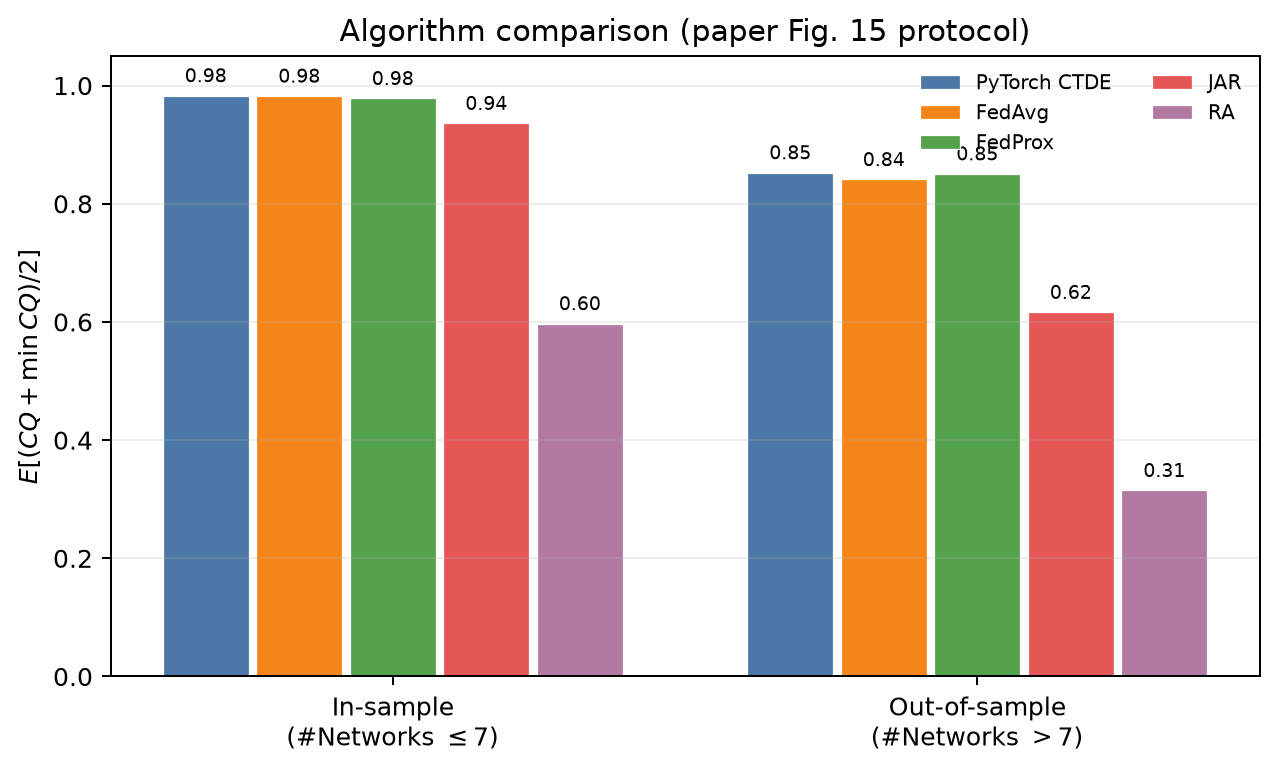
\includegraphics[width=\columnwidth]{campaign/fig15_composite_bars.png}
\caption{In-sample versus out-of-sample composite channel quality
$\mathbb{E}[(\mathrm{CQ}+\min_{\mathrm{CQ}})/2]$. In-sample: $N\leq 7$;
out-of-sample: $N>7$.}
\label{fig:fig15_bars}
\end{figure}

\begin{figure}[!t]
\centering
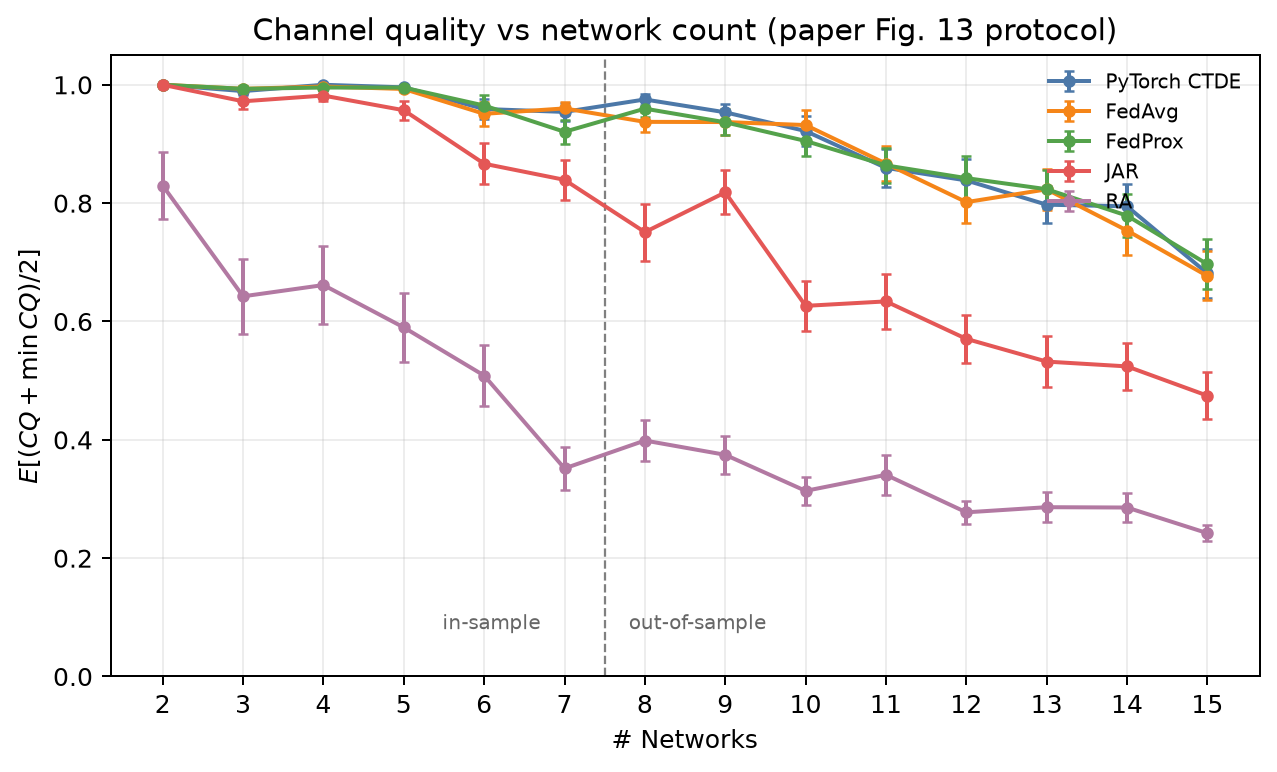
\includegraphics[width=\columnwidth]{campaign/fig13_composite_vs_n.png}
\caption{Composite channel quality versus number of networks. The dashed line
marks the training support $N\leq 7$.}
\label{fig:fig13_curves}
\end{figure}

The in-sample result is the central one. Fig.~\ref{fig:fig15_bars} shows
the PyTorch CTDE baseline at $0.983$, with \FedAvg{} and \FedProx{} at
$0.982$ and $0.978$---matching the centralized learner to within the metric
resolution, and matching the $0.98$ reported for \CARLTON{} and the $0.99$
graph-coloring bound in~\cite{cohen2024carlton}. Federated training therefore
keeps pace with pooled-experience CTDE on the domain it was trained on, while
never pooling raw sensing data and while learning from a strictly local reward
($\rho=1$). This is the expected best case: aggregating parameters instead of
experience cannot create information that pooled training does not already
have, so staying within a fraction of a percent of CTDE---not surpassing
it---is the meaningful outcome.

Fig.~\ref{fig:fig13_curves} resolves the same comparison as a function of $N$.
CTDE leads by a thin margin across most of the sweep, and both federated
methods stay well above JAR and RA for every network count. Out-of-sample
($N>7$) the all-sample gap remains small: CTDE attains a composite of
$0.853$ against $0.851$ for \FedProx{} and $0.841$ for \FedAvg{}. Federation
thus retains the same operating regime as CTDE under generalization to network
counts never seen in training, without claiming an information-theoretic
advantage over the centralized learner.

The remaining metrics of Subsection~\ref{subsec:exp_metrics} complete the
picture. Averaged over the sweep, CTDE, \FedAvg{}, and \FedProx{} all attain
$\mathrm{WS}$ near $0.931$, above $0.910$ for JAR and $0.818$ for RA. Their
convergence-time scores ($0.931$--$0.933$) sit just below JAR ($0.945$) and RA
($0.960$)---both of which converge quickly only because they barely move.
\OURS{} therefore reaches near-CTDE channel quality without paying for it in
spectrum mobility, and without needing the post-processing threshold
$\varphi$ that~\cite{cohen2024carlton} introduces to recover convergence time.

Finally, we caution against reading the training-reward gap of
Subsection~\ref{subsec:exp_reward} as evidence that federation is the stronger
learner. Reward is the surrogate that DeepMellow optimizes, and the federated
and centralized runs optimize it under different $\rho$; the operational claim
of this paper rests on Figs.~\ref{fig:fig15_bars}--\ref{fig:fig13_curves},
where CTDE is slightly ahead overall and \OURS{} remains competitive under a
strictly stronger privacy constraint.

%==============================================================================
\section{Conclusion}
\label{sec:conclusion}
%==============================================================================

We presented \OURS{}, a federated deep reinforcement learning framework for
SINR-aware distributed dynamic channel allocation under inter-carrier
interference. By replacing the global replay memory of CTDE with private,
persistent per-client buffers and aggregating only model parameters via
\FedAvg{} or \FedProx{}, the framework removes the need to export raw sensing
histories while retaining a fully decentralized execution phase. Over $30$
seeds, federated training reaches inference rewards of approximately $86.5$--
$86.6$ (ceiling $88$) under a strictly local reward ($\rho=1$). On the
channel-quality metrics $\mathbb{E}[(\mathrm{CQ}+\min\mathrm{CQ})/2]$ and WS,
evaluated over $420$ games per method against RA, JAR, and a PyTorch CTDE
baseline, the centralized learner remains slightly ahead
($0.909$ versus $0.905$ all-sample composite), while \OURS{} stays in the same
regime without sharing raw sensing data. Federation is therefore a practical
path to data sovereignty in this setting, trading a thin margin against CTDE
for a strictly stronger privacy constraint.
%==============================================================================
\begin{thebibliography}{99}

\bibitem{cohen2024carlton}
Y.~Cohen, T.~Gafni, R.~Greenberg, and K.~Cohen,
``SINR-aware deep reinforcement learning for distributed dynamic channel
allocation in cognitive interference networks,''
\emph{arXiv preprint arXiv:2402.17773}, 2024.

\bibitem{mishra2006overlapped}
A.~Mishra, V.~Shrivastava, S.~Banerjee, and W.~Arbaugh,
``Partially overlapped channels not considered harmful,''
in \emph{Proc. ACM SIGMETRICS}, 2006, pp.~63--74.

\bibitem{blum2003metaheuristics}
C.~Blum and A.~Roli,
``Metaheuristics in combinatorial optimization: Overview and conceptual
comparison,'' \emph{ACM Computing Surveys}, vol.~35, no.~3, pp.~268--308, 2003.

\bibitem{naparstek2019deep}
O.~Naparstek and K.~Cohen,
``Deep multi-user reinforcement learning for distributed dynamic spectrum
access,'' \emph{IEEE Trans. Wireless Commun.}, vol.~18, no.~1, pp.~310--323,
2019.

\bibitem{adeogun2023distributed}
R.~Adeogun and G.~Berardinelli,
``Distributed channel allocation for mobile 6G subnetworks via multi-agent deep
Q-learning,'' in \emph{Proc. IEEE Wireless Communications and Networking
Conference (WCNC)}, 2023, pp.~1--6.

\bibitem{kaur2023deep}
A.~Kaur, J.~Thakur, M.~Thakur, K.~Kumar, A.~Prakash, and R.~Tripathi,
``Deep recurrent reinforcement learning-based distributed dynamic spectrum
access in multichannel wireless networks with imperfect feedback,''
\emph{IEEE Trans. Cogn. Commun. Netw.}, vol.~9, no.~2, pp.~281--292, 2023.

\bibitem{du2022multi}
X.~Du \emph{et al.},
``Multi-agent reinforcement learning for dynamic resource management in 6G in-X
subnetworks,'' \emph{IEEE Trans. Wireless Commun.}, vol.~22, no.~3,
pp.~1900--1914, 2022.

\bibitem{kim2019deepmellow}
S.~Kim, K.~Asadi, M.~Littman, and G.~Konidaris,
``DeepMellow: Removing the need for a target network in deep Q-learning,''
in \emph{Proc. Int. Joint Conf. Artificial Intelligence (IJCAI)}, 2019,
pp.~2733--2739.

\bibitem{asadi2017alternative}
K.~Asadi and M.~L. Littman,
``An alternative softmax operator for reinforcement learning,''
in \emph{Proc. Int. Conf. Machine Learning (ICML)}, 2017, pp.~243--252.

\bibitem{goldsmith2005wireless}
A.~Goldsmith,
\emph{Wireless Communications}.
Cambridge, U.K.: Cambridge Univ. Press, 2005.

\bibitem{egli1957radio}
J.~J. Egli,
``Radio propagation above 40 Mc over irregular terrain,''
\emph{Proc. IRE}, vol.~45, no.~10, pp.~1383--1391, 1957.

\bibitem{cohen2017distributed}
K.~Cohen, A.~Nedi\'{c}, and R.~Srikant,
``Distributed learning algorithms for spectrum sharing in spatial random access
wireless networks,'' \emph{IEEE Trans. Autom. Control}, vol.~62, no.~6,
pp.~2854--2869, 2017.

\bibitem{mcmahan2017fedavg}
B.~McMahan, E.~Moore, D.~Ramage, S.~Hampson, and B.~A. y~Arcas,
``Communication-efficient learning of deep networks from decentralized data,''
in \emph{Proc. Int. Conf. Artificial Intelligence and Statistics (AISTATS)},
2017, pp.~1273--1282.

\bibitem{kairouz2021advances}
P.~Kairouz \emph{et al.},
``Advances and open problems in federated learning,''
\emph{Foundations and Trends in Machine Learning}, vol.~14, no.~1--2,
pp.~1--210, 2021.

\bibitem{arjoune2019comprehensive}
Y.~Arjoune and N.~Kaabouch,
``A comprehensive survey on spectrum sensing in cognitive radio networks: Recent
advances, new challenges, and future research directions,''
\emph{Sensors}, vol.~19, no.~1, p.~126, 2019.

\bibitem{sutton2018reinforcement}
R.~S. Sutton and A.~G. Barto,
\emph{Reinforcement Learning: An Introduction}, 2nd~ed.
Cambridge, MA, USA: MIT Press, 2018.

\bibitem{he2015delving}
K.~He, X.~Zhang, S.~Ren, and J.~Sun,
``Delving deep into rectifiers: Surpassing human-level performance on
ImageNet classification,''
in \emph{Proc. IEEE Int. Conf. Computer Vision (ICCV)}, 2015, pp.~1026--1034.

\bibitem{li2020fedprox}
T.~Li, A.~K. Sahu, M.~Zaheer, M.~Sanjabi, A.~Talwalkar, and V.~Smith,
``Federated optimization in heterogeneous networks,''
in \emph{Proc. Machine Learning and Systems (MLSys)}, vol.~2, 2020,
pp.~429--450.

\end{thebibliography}

\end{document}
